
\documentclass[border={10pt 10pt 10pt 10pt},varwidth]{standalone}
\usepackage{amsmath}
\usepackage{tikz} 
\usetikzlibrary{calc,intersections,through,backgrounds,decorations.pathmorphing, decorations.shapes,decorations.markings,patterns,decorations.pathreplacing,calligraphy}
%include other needed packages here   

\DeclareMathOperator{\supp}{supp}
\DeclareMathOperator{\dist}{dist}
\DeclareMathOperator{\vol}{vol}
\DeclareMathOperator{\diag}{diag}
\DeclareMathOperator{\tr}{tr}
\DeclareMathOperator{\Img}{\operatorname{Im}}
\DeclareMathOperator{\Id}{\operatorname{Id}}
\DeclareMathOperator{\Rep}{\operatorname{Rep}}
\DeclareMathOperator{\Mod}{\operatorname{mod}}
\DeclareMathOperator{\Hom}{\operatorname{Hom}}
\DeclareMathOperator{\Ext}{\operatorname{Ext}}
\DeclareMathOperator{\Mor}{\operatorname{Mor}}
\DeclareMathOperator{\rad}{\operatorname{rad}}
\DeclareMathOperator{\ind}{\operatorname{ind}}
\DeclareMathOperator{\End}{\operatorname{End}}
\DeclareMathOperator{\Jac}{\operatorname{Jac}}
\DeclareMathOperator{\Spec}{\operatorname{Spec}}
\DeclareMathOperator{\Modup}{\overline{\operatorname{mod}}}
\DeclareMathOperator{\Moddown}{\underline{\operatorname{mod}}}
\DeclareMathOperator{\Homup}{\overline{\operatorname{Hom}}}
\DeclareMathOperator{\Homdown}{\underline{\operatorname{Hom}}}
\DeclareMathOperator{\gldim}{\operatorname{gl.dim}}
\DeclareMathOperator{\projdim}{\operatorname{proj.dim}}
\DeclareMathOperator{\injdim}{\operatorname{inj.dim}}
\DeclareMathOperator{\dimv}{\operatorname{\underline{\mathbf{dim}}}}


\DeclareMathOperator{\Flagd}{\operatorname{Flag}_{d}}
\DeclareMathOperator{\Flagdstr}{\operatorname{Flag}_{d,str}}
\newcommand{\Gr}{\operatorname{Gr}}
\newcommand{\Grr}{\operatorname{Gr}}
\newcommand{\Gralg}[1]{\operatorname{Gr}^{#1}}
\newcommand{\Grq}{\operatorname{Gr}^{KQ}}
\newcommand{\Flag}{\operatorname{Flag}}
\newcommand{\Flagstr}[1]{\operatorname{Flag}_{#1,str}}
\newcommand{\dimvec}[1]{\boldsymbol{#1}}
\newcommand{\ord}{\operatorname{ord}}
\newcommand{\orde}{\operatorname{ord}_e }
\newcommand{\ftdimvec}[1]{\underline{\dimvec{#1}}}
\newcommand{\representation}[2]{\genfrac{}{}{0pt}{3}{\phantom{000}#2\phantom{00}}{#1}}
\begin{document}
%https://latexdraw.com/how-to-draw-curly-braces-in-tikz/
\begin{center}
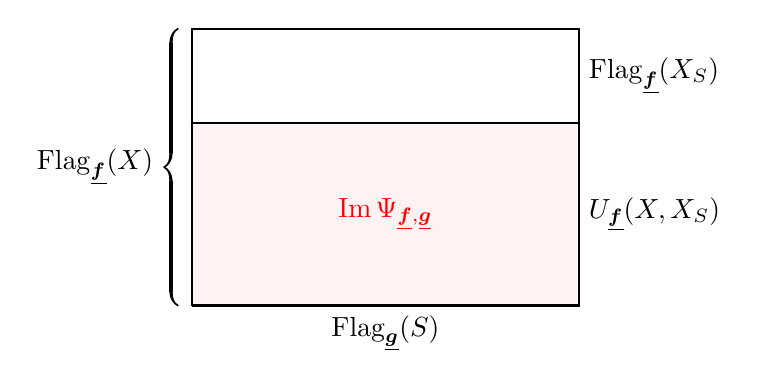
\begin{tikzpicture}[x=2em, y=2em]
\def\a{0}
\filldraw[thick, black, fill=red!5]
    (12+\a,0)--(12+\a,5)--(19+\a,5)--(19+\a,0)--(12+\a,0);
\filldraw[thick, black, fill=white]
    (12+\a,3.3)--(12+\a,5)--(19+\a,5)--(19+\a,3.3)--(12+\a,3.3);
\draw 
    (15.5+\a,1.65) node {\textcolor{red}{$\displaystyle\Img \Psi_{\ftdimvec{f},\ftdimvec{g}}$}}
    (19+\a,4.15) node[anchor=west] {$\Flag_{\ftdimvec{f}}(X_S)$}
    (19+\a,1.65) node[anchor=west] {$U_{\ftdimvec{f}}(X,X_S)$}      
    (15.5+\a,0) node[anchor=north] {$\Flag_{\ftdimvec{g}}(S)$};
\draw [very thick,decorate,
    decoration = {calligraphic brace,raise=5pt,
            amplitude=5pt}] (12+\a,0) --  (12+\a,5)
            node[pos=0.5,left=10pt,black]{$\Flag_{\ftdimvec{f}}(X)$};    
\end{tikzpicture}
\end{center}
\end{document}